\chapter{System implementation with Robot controller module}
\indent This chapter describes how all of components mentioned above are assembled. In design, I apply top-down approach in system development process. First, system is broken down into modules in which each system's function is handled separately. Next, functions of modules are presented in groups of communicating interfaces and groups of internal processing methods. Consequently, modules is divided into smaller and more dedicated units.

For each module, design pattern is engaged correspondingly to its operation behavior for the sake of ease in maintenance and convenience for extensibility.

Finally, when the system walking through all unit test cases, it is connected with the Delta robot to accomplish desired activities.

\section{System implementation}
\subsection{Whole system class diagram}
    \begin{figure}[H]
		\centering
		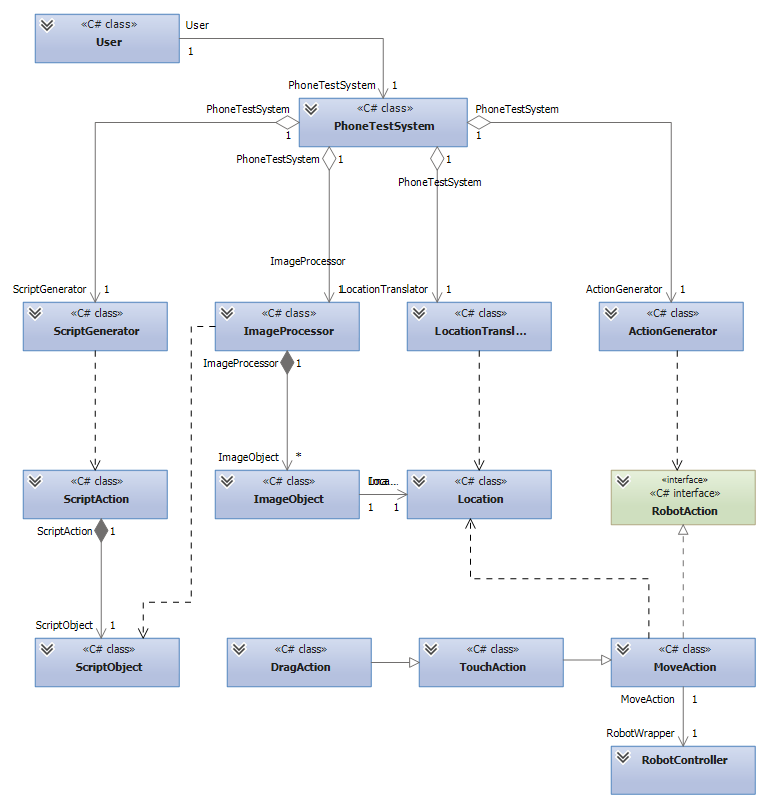
\includegraphics[scale=0.75]{Chapters/Fig/class_diagram.png}
		\caption{System class diagram}
		\label{fig:class_diagram}
	\end{figure}

\subsection{Main components of the system}
	\begin{figure}[H]
		\centering
		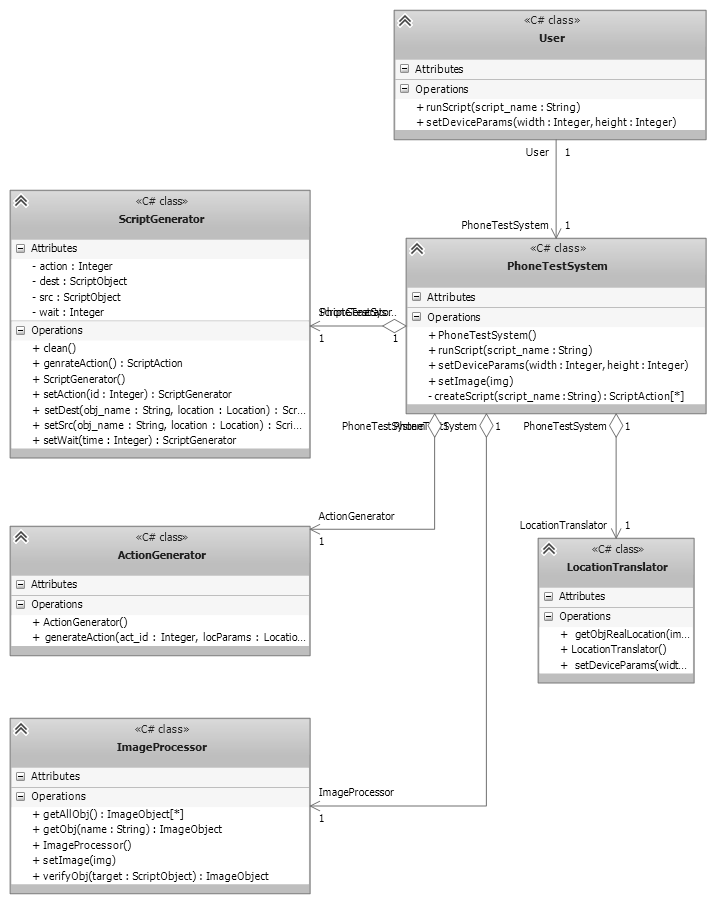
\includegraphics[scale=0.75]{Chapters/Fig/main_class.png}
		\caption{System main components}
		\label{fig:main_class}
	\end{figure}

\subsection{Script Generator structure}
	\begin{figure}[H]
		\centering
		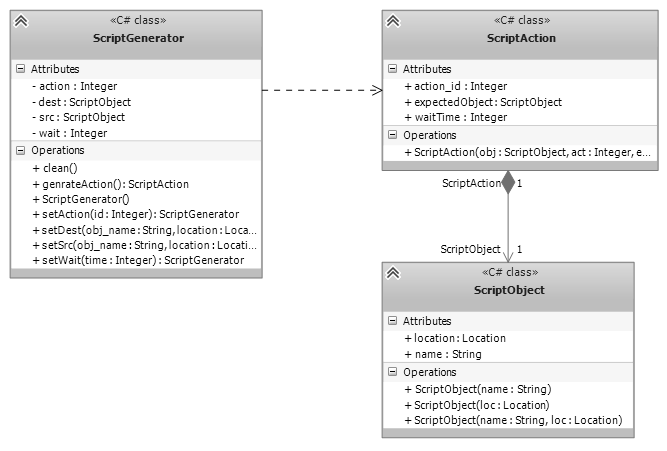
\includegraphics[scale=0.75]{Chapters/Fig/script_gen.png}
		\caption{Script Generator structure}
		\label{fig:script_gen}
	\end{figure}

\subsection{Image Processor structure}
	\begin{figure}[H]
		\centering
		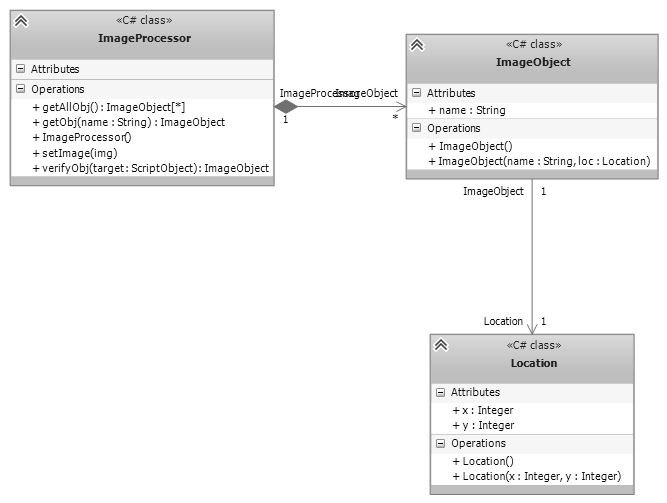
\includegraphics[scale=0.75]{Chapters/Fig/img_processor.png}
		\caption{Image Processor structure}
		\label{fig:img_processor}
	\end{figure}

\subsection{Action Generator structure}
	\begin{figure}[H]
		\centering
		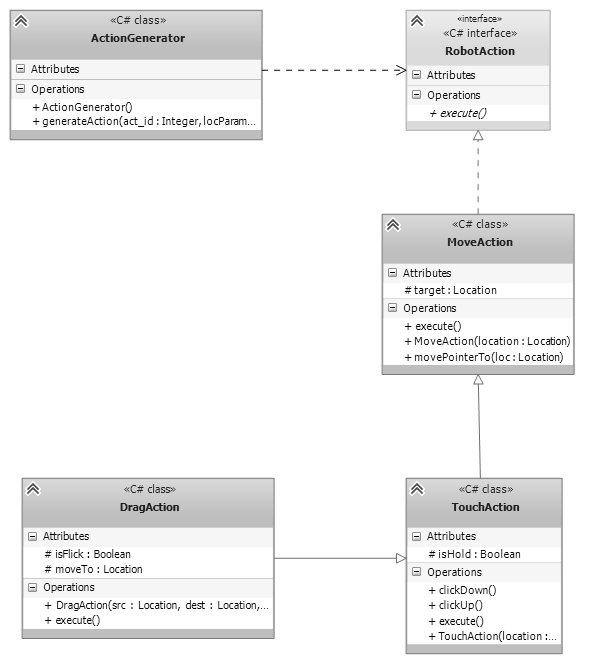
\includegraphics[scale=0.75]{Chapters/Fig/act_gen.png}
		\caption{Action Generator structure}
		\label{fig:act_gen}
	\end{figure}

\section{Robot interface command}
	\begin{itemize}
		\item[--] GotoXYZ
		\item[--] MoveToDest
		\item[--] ClickUp
		\item[--] ClickDown
	\end{itemize}

